\documentclass[a4paper, 20pt]{article}
\usepackage[english]{babel}
\usepackage{amsmath}
\usepackage{graphicx}
\usepackage{subcaption}
\usepackage{placeins}
\usepackage[T1]{fontenc}
\usepackage[utf8]{inputenc}
\usepackage{floatrow}

\author{Maarten de Jonge \\
    Inge Becht}
\date{\today}
\title{Assignment 2\\ 
Making a range finder using an omni-directional camera }

\begin{document}
\maketitle

This assignment was about making a range finder using an omni-directional
camera on a Lego robot. 
Because most of the code was already given in the assignment, the report
mostly consists of experimenting with values for different variables to
create the best possible mapping of the camera visualisation and the real world.
In the end a map of the environment will be shown using the parameters that were
found to be optimal.

\section{The steps towards simulating a range finder}

The first step towards creating the final map is calibrating the camera. For
this purpose the script \texttt{calibrate\_camera\_offline.m} was modified to
work with a single picture taken from the omnidirectional camera, as shown in
figure \ref{fig:snapshot}.

\begin{figure}[!ht]
\centering
  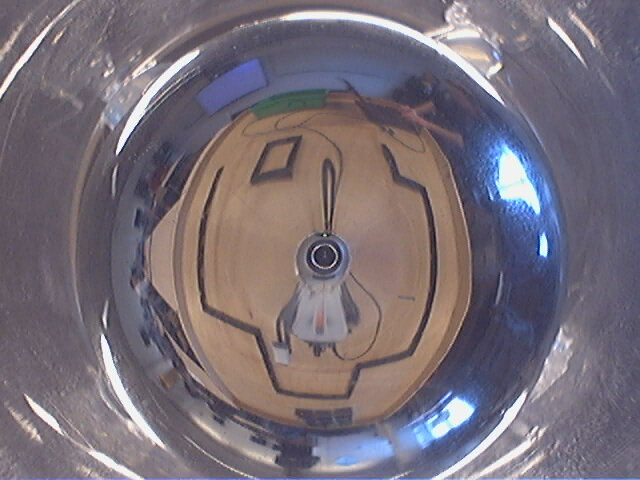
\includegraphics[width=0.5\textwidth]{omni_snapshot.jpg}
  \label{fig:snapshot}
  \caption{A snapshot from the omnidirectional camera}
\end{figure}

Calibration values were set: $Rmin = 77$ , $Rmax = 160$, $Centre\_x = 325.2203$ and
$Centre\_y =  225.0$

This created the areas seen in figure \ref{fig:circles}, where the area between the
outer pink circle and
the inner pink circle is considered `useful information'. Figure
\ref{fig:straight} shows the same image, except unwrapped from the center.

\begin{figure}[!ht]
\centering
\begin{floatrow}
  \ffigbox[\FBwidth]{\caption{Circle indicating used mirror space}\label{fig:circles}}{
  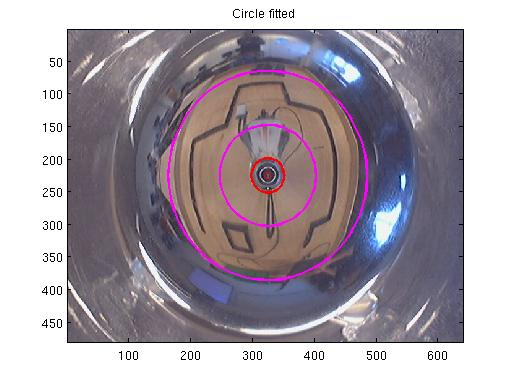
\includegraphics[width=0.5\textwidth]{map_images/camera_spaces.jpg}}
  
  \ffigbox[\FBwidth]{\caption{Flipped and straightened image} \label{fig:straight}}{
  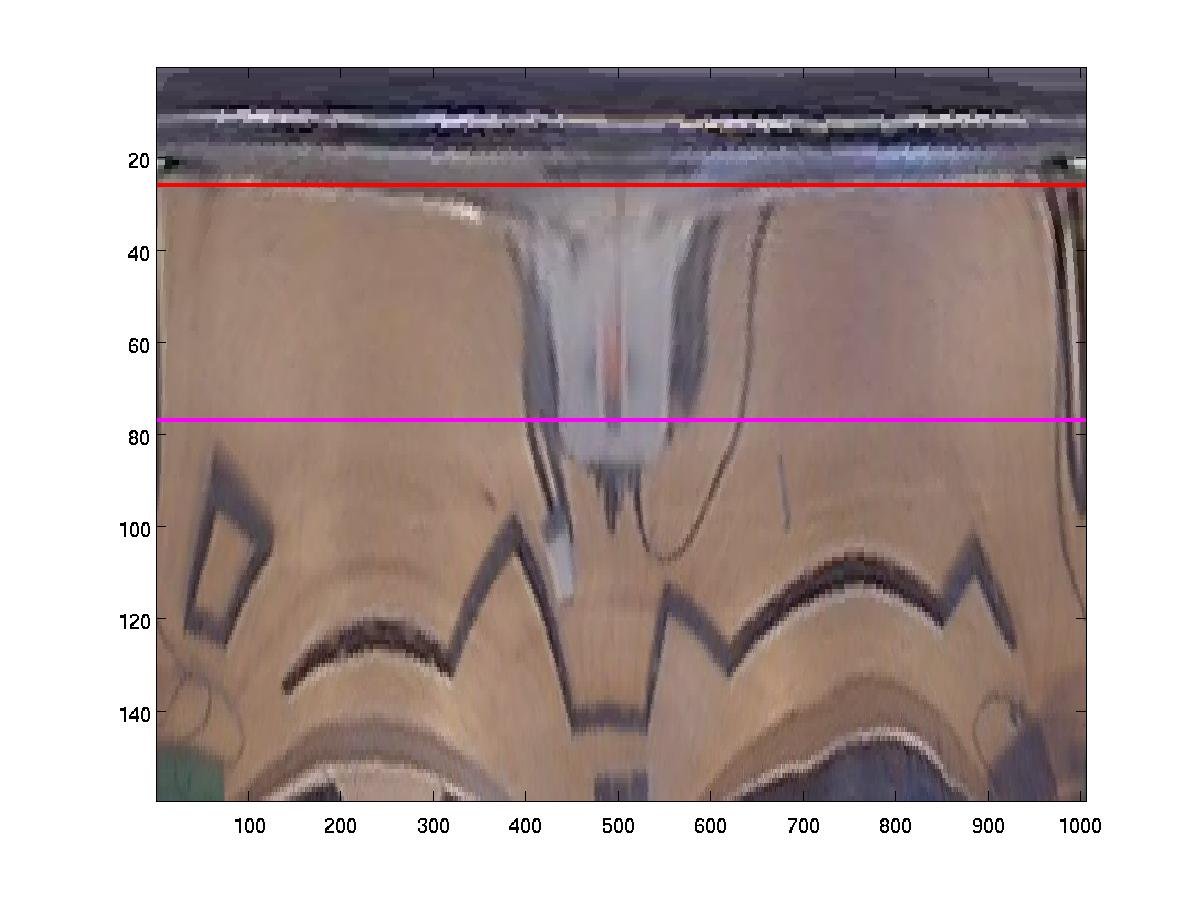
\includegraphics[width=0.5\textwidth]{map_images/straightened_image.jpg}}
\end{floatrow}
\end{figure}

To extract the walls from the original image, it needs to be unwarped and all
data that does not fall between the two pink lines in \ref{fig:circles} needs to
be thrown away. The premade \texttt{imunwrap.m} script does exactly this. It
takes a new parameter $angstep$ which determines the angular resolution of the
simulated laser scanner. The bigger the angle the worse the resolution is, as
can be seen in figure \ref{fig:angstep0.05} and \ref{fig:angstep5}.

\begin{figure}[!ht]
\centering
\begin{floatrow}
    \ffigbox[\FBwidth]{\caption{\texttt{imunwrap.m} applied with angstep = 0.05}\label{fig:angstep0.05}}{
  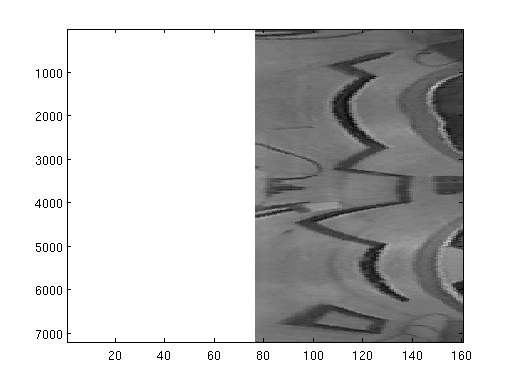
\includegraphics[width=0.5\textwidth]{rectangle_0_05.png}}
  
  \ffigbox[\FBwidth]{\caption{\texttt{imunwrap.m} applied with angstep =5}
  \label{fig:angstep5}}{
  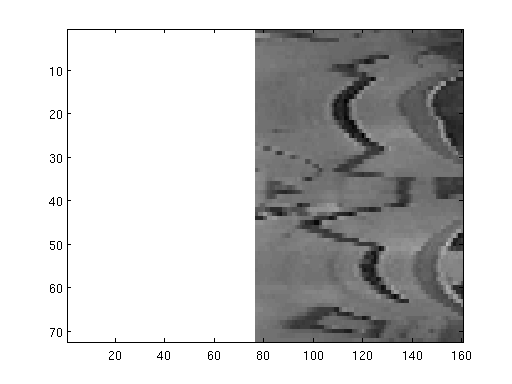
\includegraphics[width=0.5\textwidth]{rectangle_5png.png}}
\end{floatrow}
\end{figure}

At first glance one might say a lower angle (thus, higher resolution) would lead
to more precision, but the problem with a higher resolution is the great amount of
detail that will be kept in the image and thus a great amount of noise that
comes with it. A too low resolution, however, could make the distance
estimation less accurate. $Angstep$ is thus one of the parameters with
wich will be experimented with to find a suitable value.

Whatever the chosen $angstep$ is, there still needs to be some more noise
reduction to accentuate the position of the wall pieces. A simple black and
white threshold is used for this. A more difficult choice is however at what
value to set the threshold, something that can not be determined from a single
image, but we still try to approximate it that way. In figure \ref{fig:thresh100} and
\ref{fig:thresh75} two different tresholds can be seen. Note that the range of
of the input grayscale image is not normalised between 0 and 1, but instead 0
and 255, leading to the threshold values of 100 and 75.

\begin{figure}[!ht]
\centering
\begin{floatrow}
    \ffigbox[\FBwidth]{\caption{Threshold = 100 applied with angstep =
    1}\label{fig:thresh100}}{
  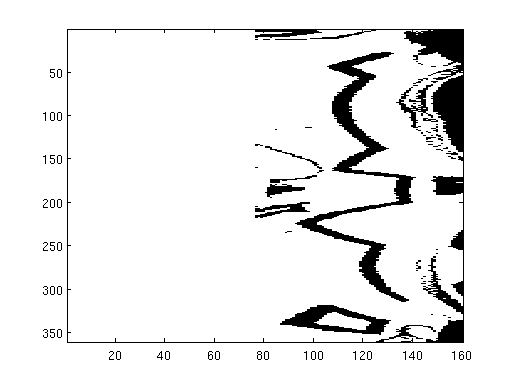
\includegraphics[width=0.5\textwidth]{black_thresh_100.png}}
  
  \ffigbox[\FBwidth]{\caption{Threshold = 75. Applied with angstep =1}
  \label{fig:thresh75}}{
  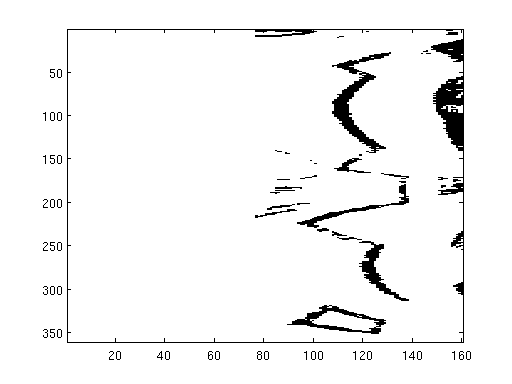
\includegraphics[width=0.5\textwidth]{black_thresh_75.png}}
\end{floatrow}
\end{figure}

The following step is to iterate through each horizontal line to scan for
transition from white to black. Using the height of the camera (around 0.33
meters) and a certain $\alpha$ the distance towards these transitions can be
calculated.  Different values for $\alpha$ were experimented with. In case of
the robot in Zurich, $\alpha$ was given the value of 95 pixels, so we experiment
around these values as well.

\subsection{Varying parameter values}
The data set with all tested values of angstep, the black and white
threshold and  $\alpha$ was created by running \texttt{create\_dataset.m} and can be run with
or without calibration. The following different combination of values were
used:\\

\begin{align*}
    angstep  \in \{0.05, 0.5, 1, 1.5, 2, 5, 10\}\\
    BWthresh \in \{75, 80, 85, 90, 95 100\}\\
    \alpha   \in \{80, 95, 100, 120, 130, 150\}\\
\end{align*}

\subsection{Varying $angstep$}

When using $BWthresh = 75 $ and $\alpha = 130$ and varying $angstep$, we get
figure \ref{fig:angstep1}, \ref{fig:angstep2}, \ref{fig:angstep3},
\ref{fig:angstep4}. Although we expected a high resolution to add noise,
in this particular testing setup it's not problem.
In case of the $angstep = 0.05$, we can identify 5 clear outliers and
in the case of $angstep =2$ only 3 less than this. It seems there might not have to
be a big trade-off between resolution and accuracy.
\begin{figure}[!ht]
\centering
\begin{floatrow}
  \ffigbox[\FBwidth]{\caption{$angstep = 0.05$ }\label{fig:angstep1}}{
  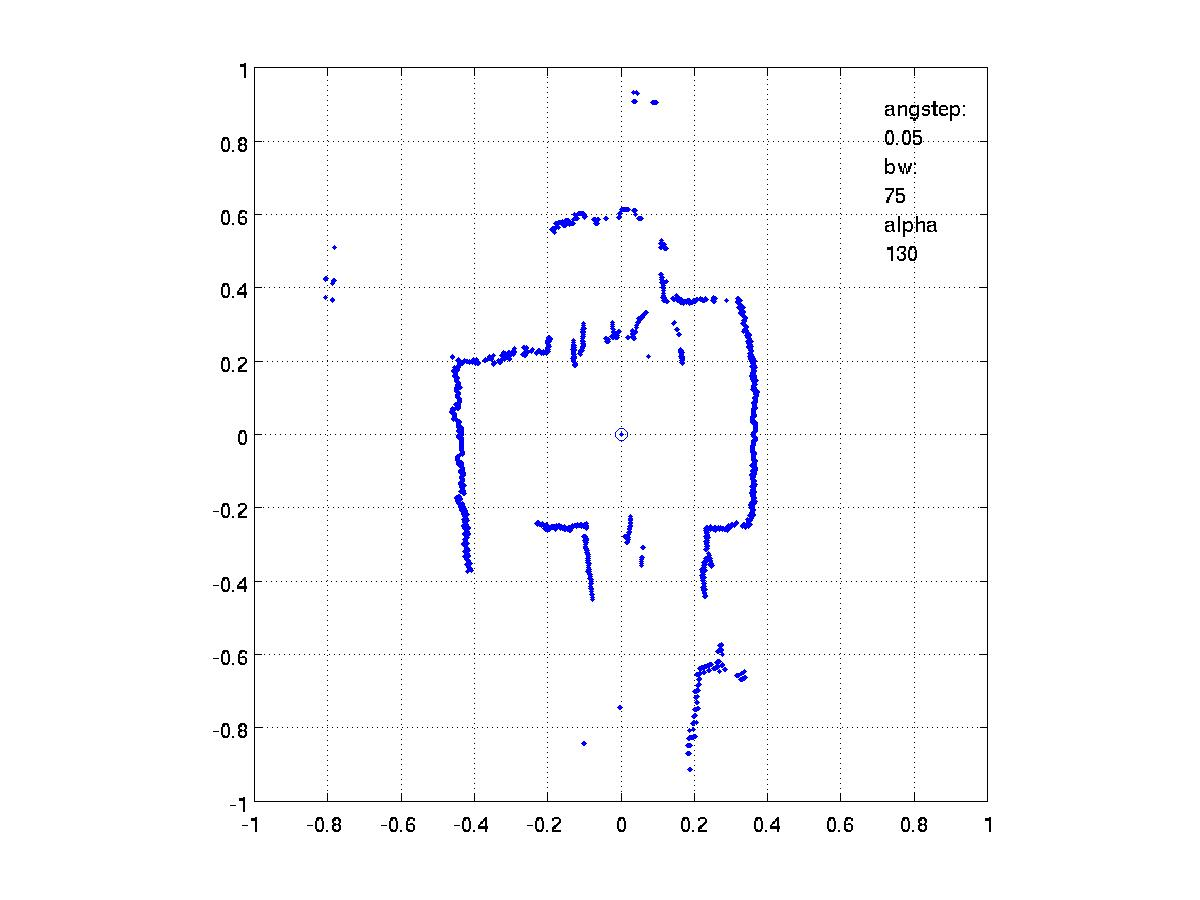
\includegraphics[width=0.7\textwidth]{fig5.jpg}}
  \ffigbox[\FBwidth]{\caption{$angstep = 0.5 $}
  \label{fig:angstep2}}{
  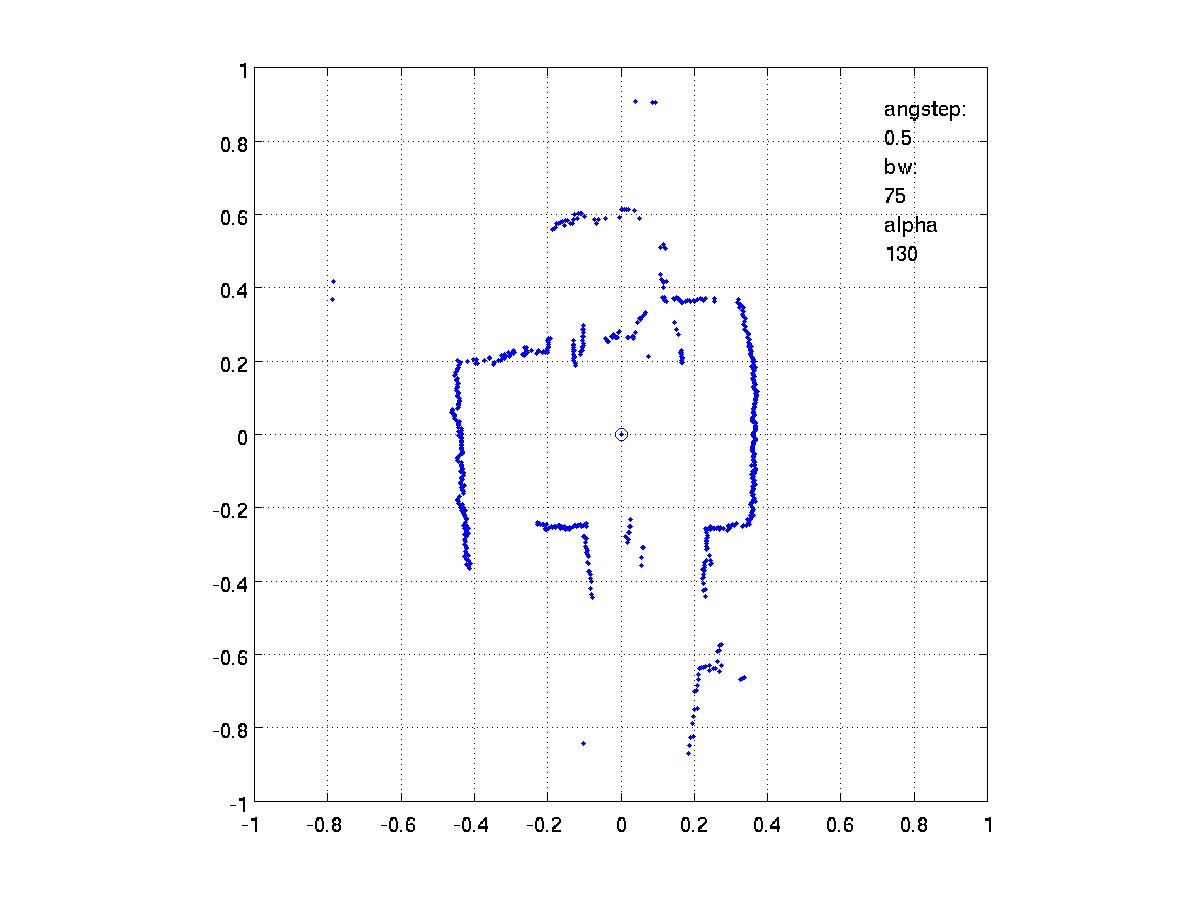
\includegraphics[width=0.7\textwidth]{fig41.jpg}}
\end{floatrow}
\end{figure}

\begin{figure}[!ht]
\centering
\begin{floatrow}
    \ffigbox[\FBwidth]{\caption{$angstep =1 $ }\label{fig:angstep3}}{
  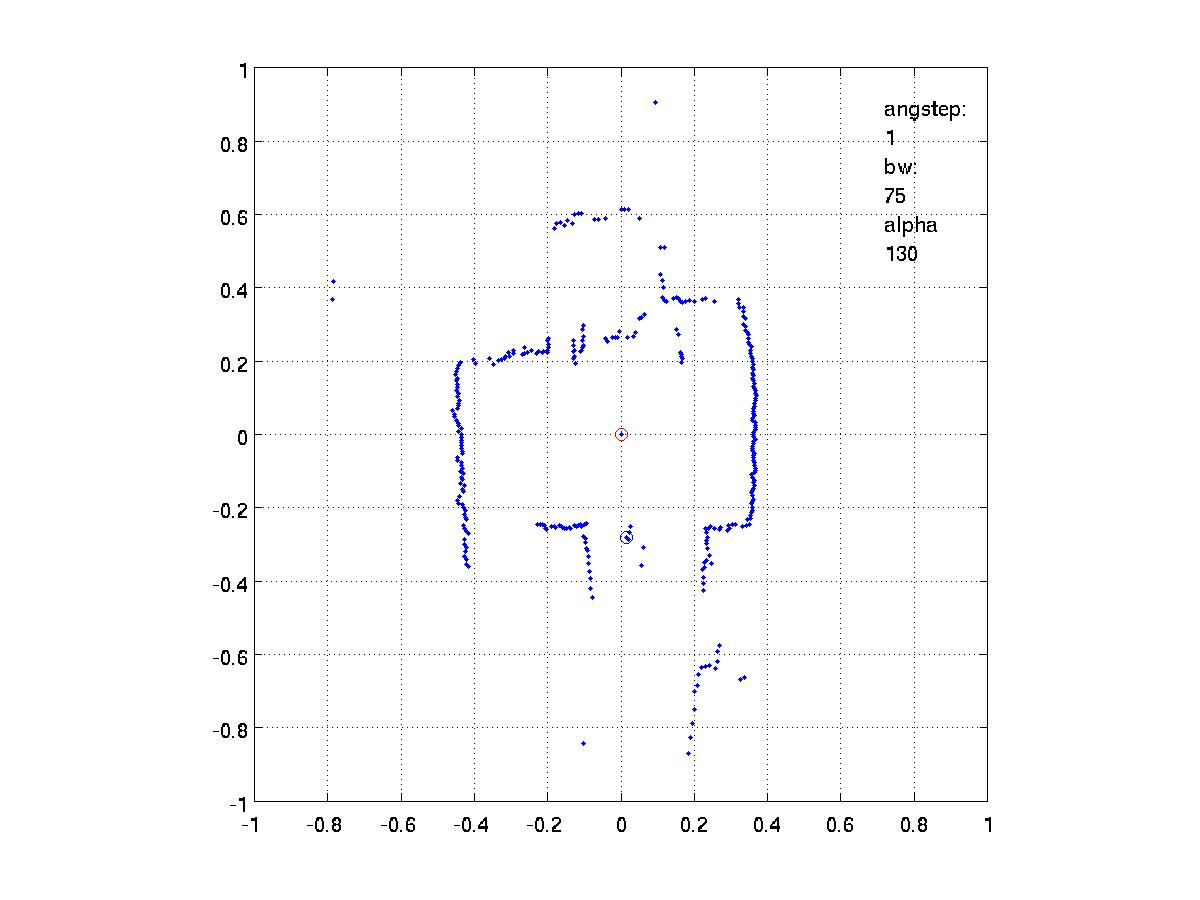
\includegraphics[width=0.7\textwidth]{fig77.jpg}}
  
  \ffigbox[\FBwidth]{\caption{$angstep = 2 $}
  \label{fig:angstep4}}{
  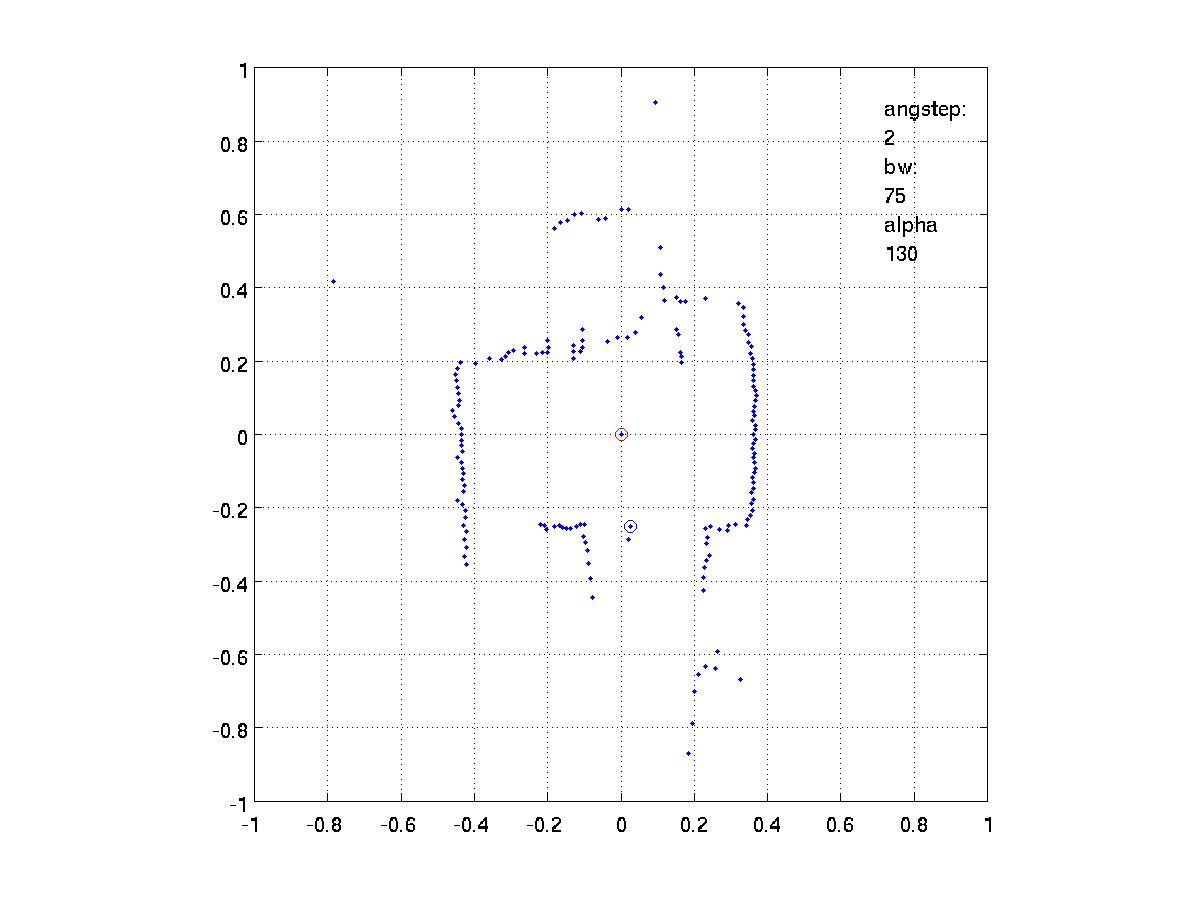
\includegraphics[width=0.7\textwidth]{fig149.jpg}}
\end{floatrow}
\end{figure}

\FloatBarrier
\subsection{Varying $BWThresh$}
When varying the values of $BWthresh$ and keeping $angstep = 0.05$ and $\alpha=
130$ we get the results seen in figure \ref{fig:bw1}, \ref{fig:bw2},
\ref{fig:bw3} and \ref{fig:bw4}. It seems that in the chosen threshold range it
does not really matter that much what value you use.
But as stated earlier, this result should be taken lightly, as it is only
constructed with a single image with only one kind of lighting condition.
Depending on the final use of the images a better threshold should be considered
\begin{figure}[!ht]
\centering
\begin{floatrow}
  \ffigbox[\FBwidth]{\caption{$BWthresh = 75$ }\label{fig:bw1}}{
  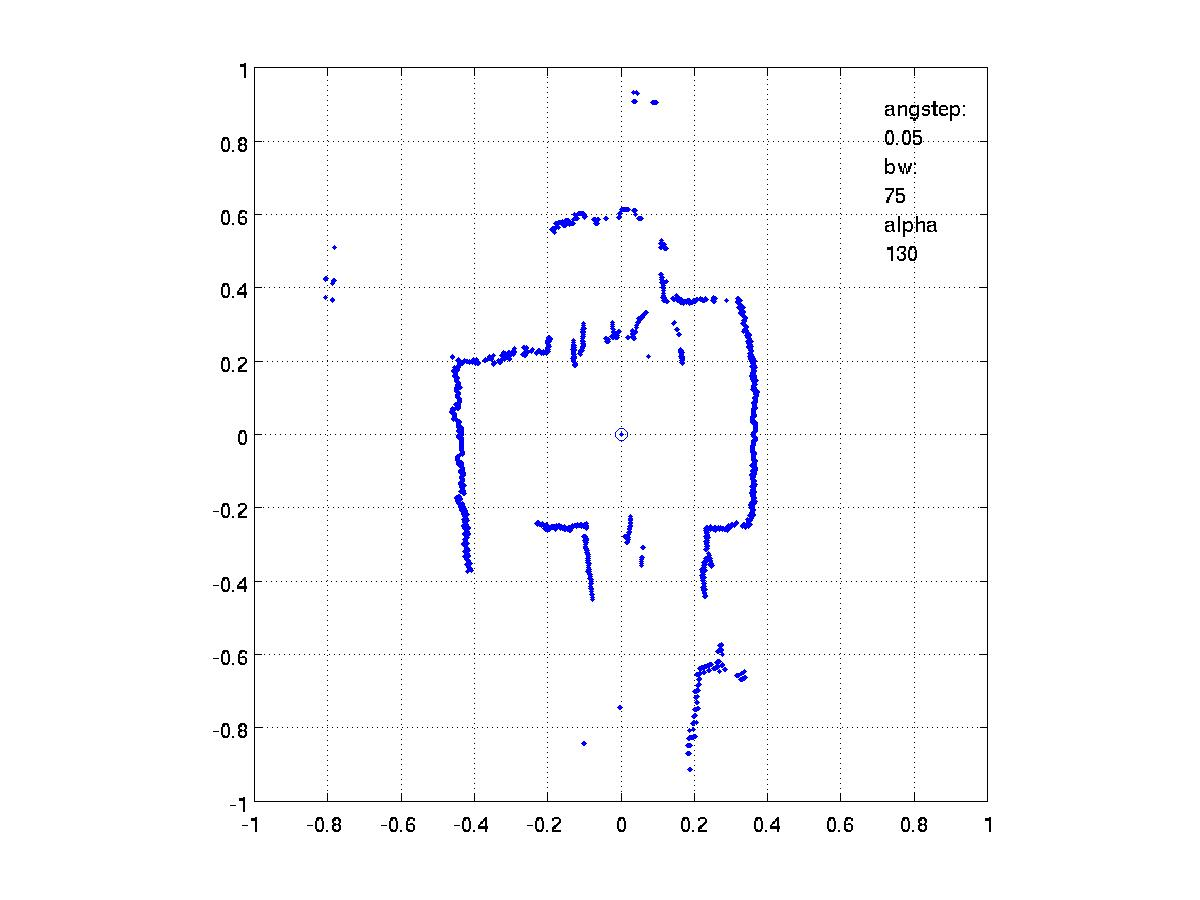
\includegraphics[width=0.7\textwidth]{fig5.jpg}}
  \ffigbox[\FBwidth]{\caption{$BWthresh = 85 $}
  \label{fig:bw2}}{
  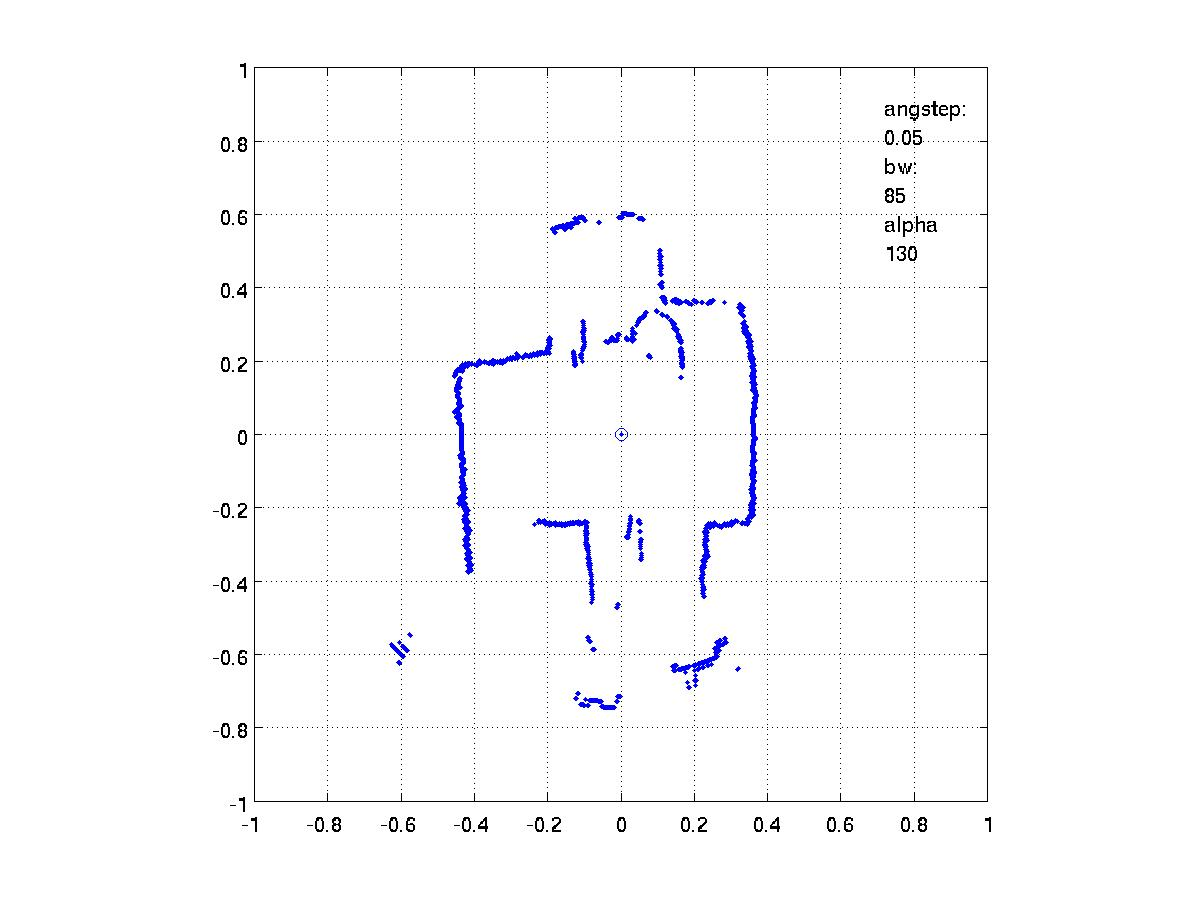
\includegraphics[width=0.7\textwidth]{fig17.jpg}}
\end{floatrow}
\end{figure}

\begin{figure}[!ht]
\centering
\begin{floatrow}
  \ffigbox[\FBwidth]{\caption{$BWthresh = 90$ }\label{fig:bw3}}{
  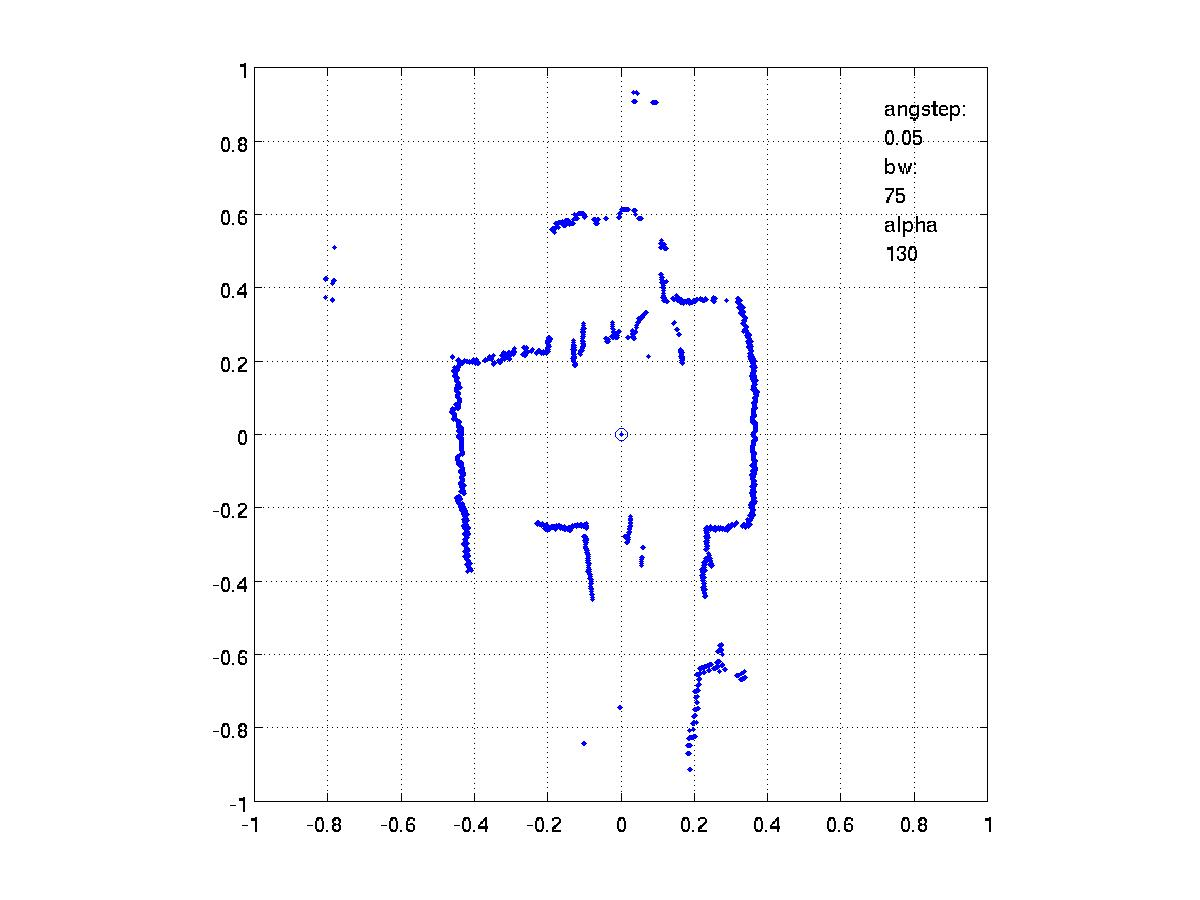
\includegraphics[width=0.7\textwidth]{fig5.jpg}}
  \ffigbox[\FBwidth]{\caption{$BWthresh = 100 $}
  \label{fig:bw4}}{
  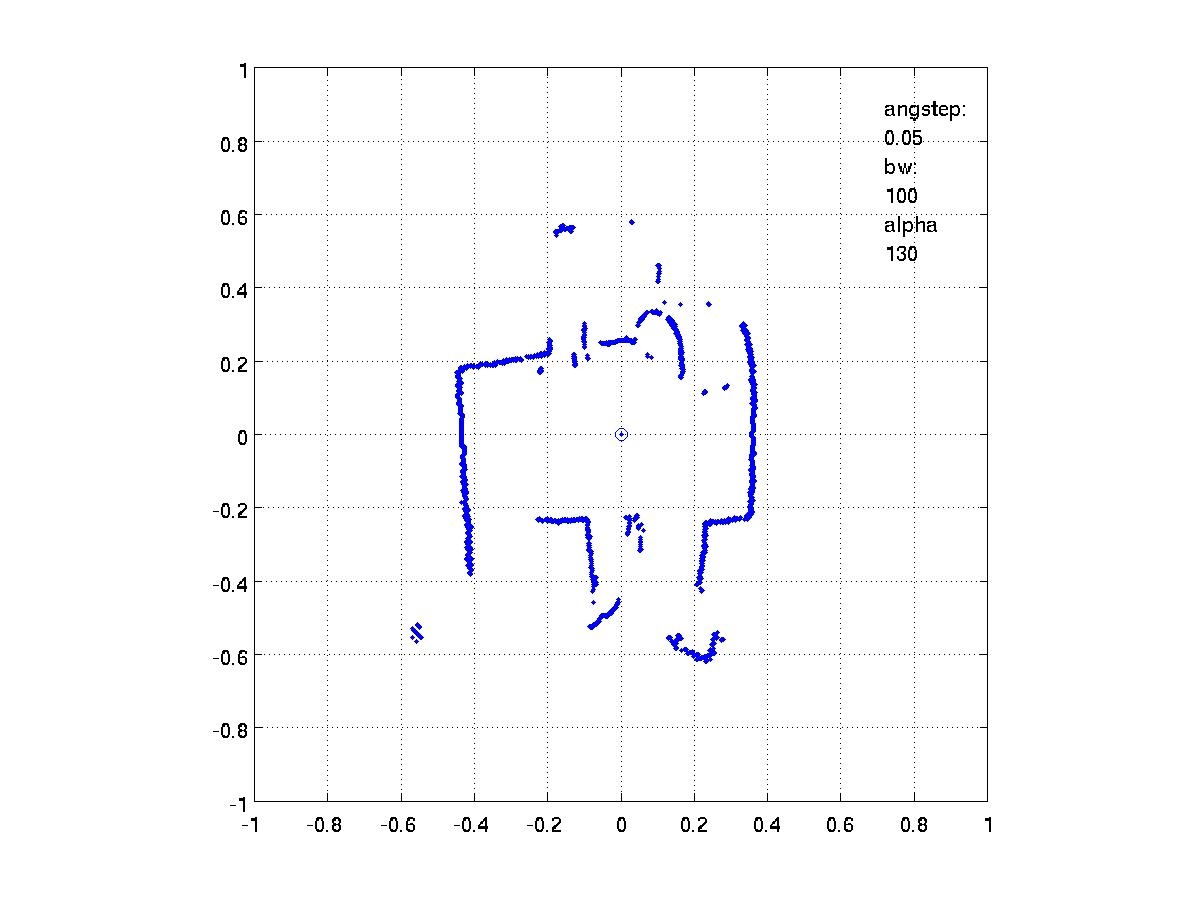
\includegraphics[width=0.7\textwidth]{fig35.jpg}}
\end{floatrow}
\end{figure}

\FloatBarrier
\subsection{Varying $\alpha$}
When varying the values of $\alpha$ and keeping $angstep = 0.05$ and $BWthresh=
80$ we get the results seen in figure \ref{fig:alpha1}, \ref{fig:alpha2}
\ref{fig:alpha3}, \ref{fig:alpha4}.These images show that $\alpha$ should not be
taken higher than 130 pixels as than the lines begin to deform in the shape of
the mirror, which has probably to do with a less than optimal calibration. This
would make it harder to do edge or line detection. Also,
the parameter should not be chosen less than 120 pixels as than the position
estiation is not all that precise.

\begin{figure}[!ht]
\centering
\begin{floatrow}
  \ffigbox[\FBwidth]{\caption{$\alpha = 95$ }\label{fig:alpha1}}{
  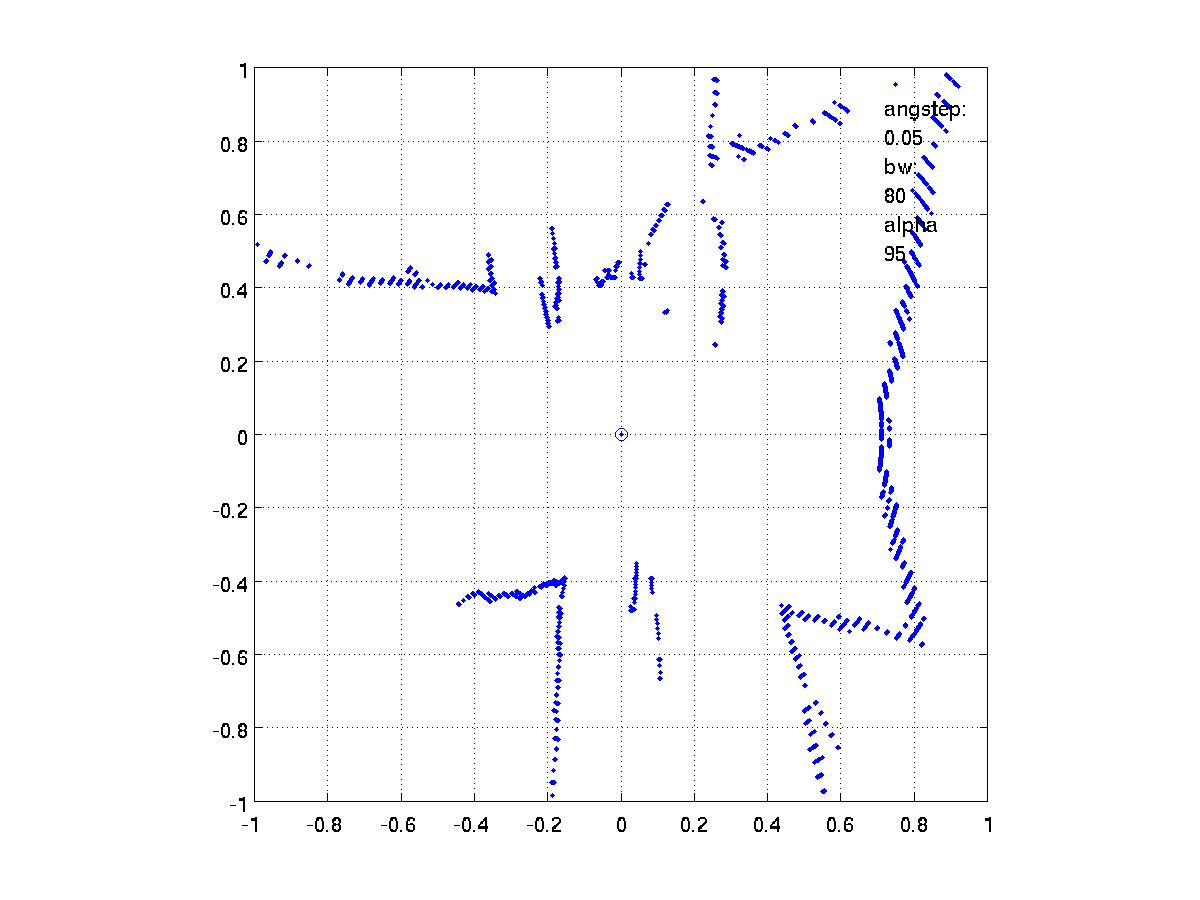
\includegraphics[width=0.7\textwidth]{fig8.jpg}}
  \ffigbox[\FBwidth]{\caption{$\alpha = 100 $}
  \label{fig:alpha2}}{
  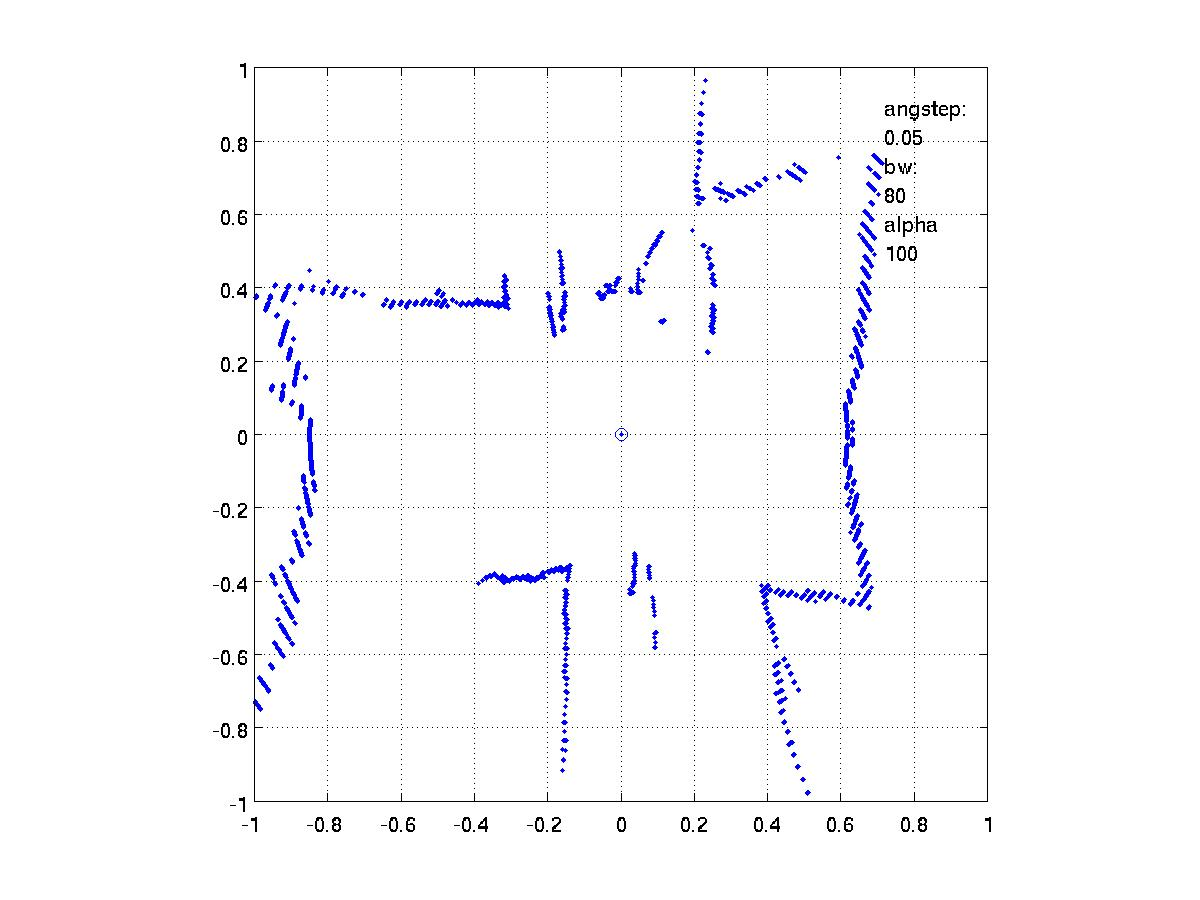
\includegraphics[width=0.7\textwidth]{fig9.jpg}}
\end{floatrow}
\end{figure}

\begin{figure}[!ht]
\centering
\begin{floatrow}
    \ffigbox[\FBwidth]{\caption{$\alpha =130 $ }\label{fig:alpha3}}{
  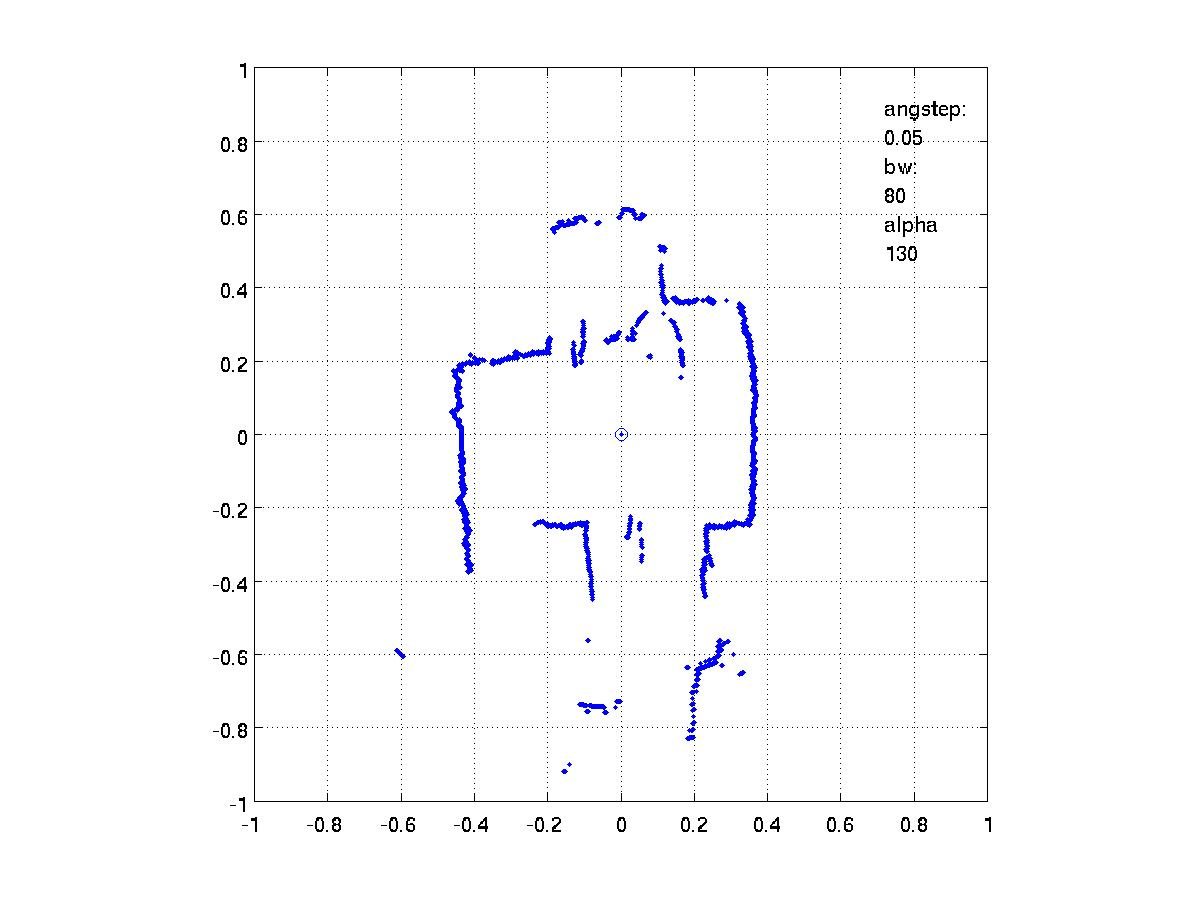
\includegraphics[width=0.7\textwidth]{fig11.jpg}}
  
  \ffigbox[\FBwidth]{\caption{$\alpha = 150 $}
  \label{fig:alpha4}}{
  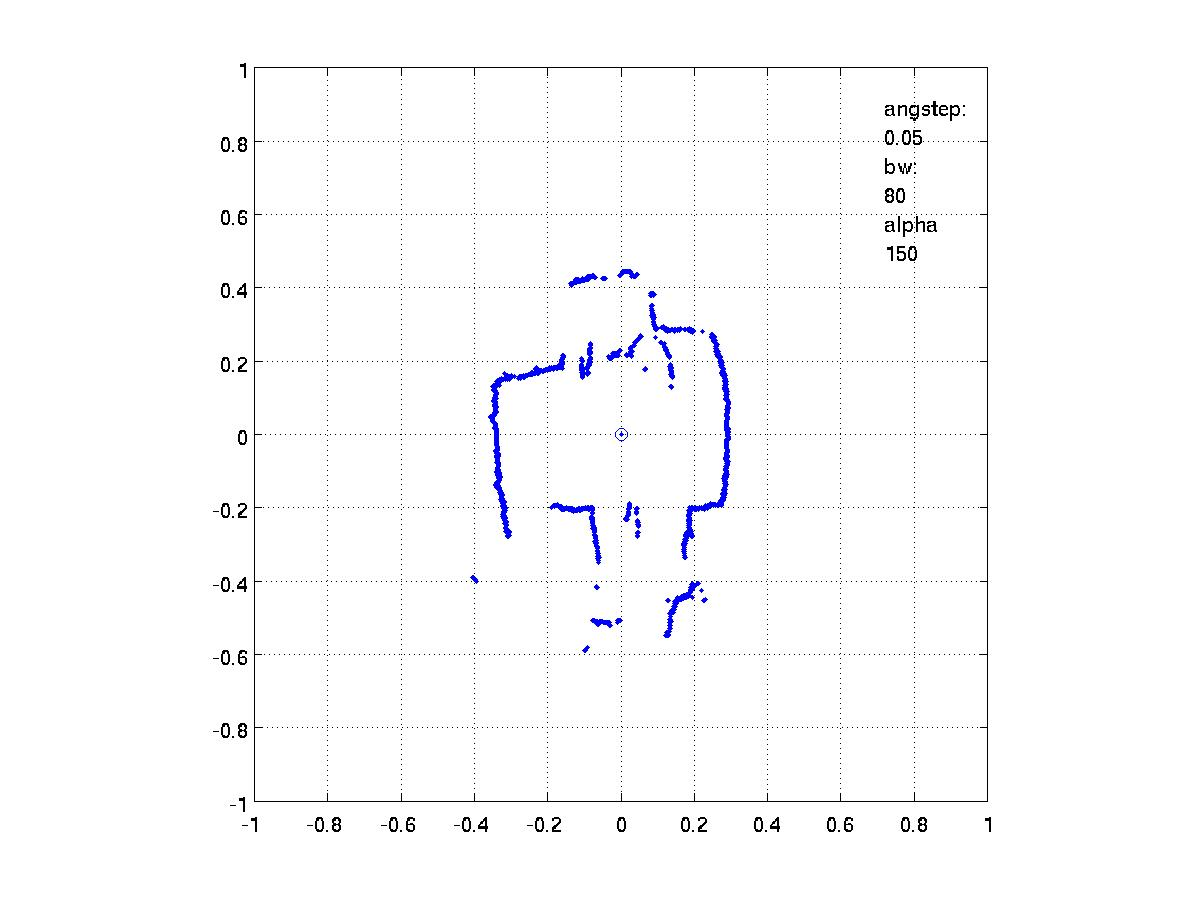
\includegraphics[width=0.7\textwidth]{fig12.jpg}}
\end{floatrow}
\end{figure}

\FloatBarrier


\subsection{Calculating the error}
So now we know that the optimal value for $angstep = 0.05$, for $\alpha = 130$
and for $BWthresh$ it does not matter in the tested threshold. This can be used for calculating the
error using function \texttt{compute\_uncertainty}. The final result of this
can be seen in figure \ref{fig:error} in case of the optimal parameters
and in figure \ref{fig:error2} in case of less than optimal parameters.
We are not sure why the camera position creates such large errors in case of
figure \ref{fig:error2}. It does not have to do with camera
calibration,
because it never happens in case of good parameter choices.

the case with ...
\begin{figure}[!ht]
\centering
\begin{floatrow}
    \ffigbox[\FBwidth]{\caption{The image showing the distance error in case of
    $\alpha = 130$, $angstep = 0.05$ and $BWthresh = 90$ }\label{fig:error}}{
  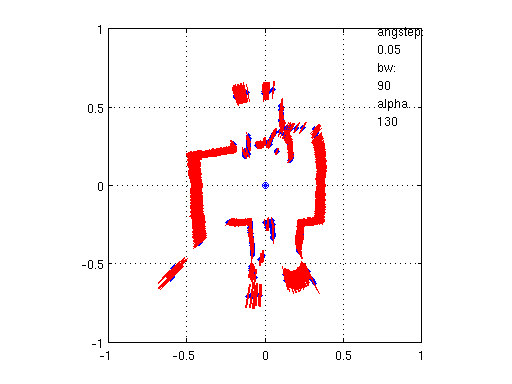
\includegraphics[width=0.7\textwidth]{error_image.png}}
  
  \ffigbox[\FBwidth]{\caption{The image showing the distance error in case
      of$\alpha = 90$, $angstep = 1$ and $BWthresh = 90$}
  \label{fig:error2}}{
  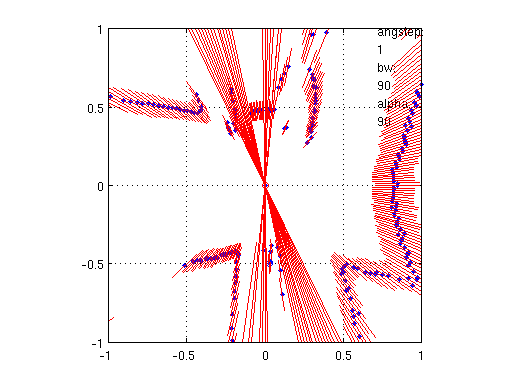
\includegraphics[width=0.7\textwidth]{error_image2.png}}
\end{floatrow}
\end{figure}

\end{document}
